\section{Evaluation}
\label{sec:evaluation}

\begin{figure*}[h]
\begin{subfigure}{0.49\textwidth}
  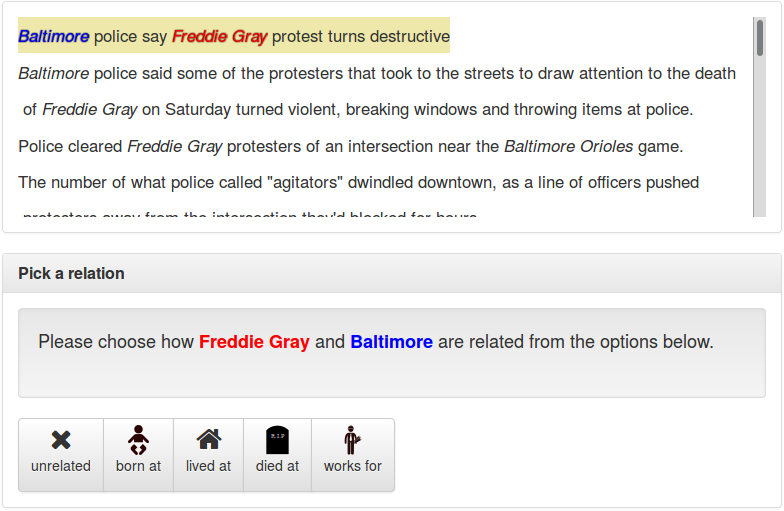
\includegraphics[width=\textwidth]{figures/relation-interface}
  \caption{\label{fig:relation-interface} Relation extraction.}
\end{subfigure}
\hfill
\begin{subfigure}{0.49\textwidth}
  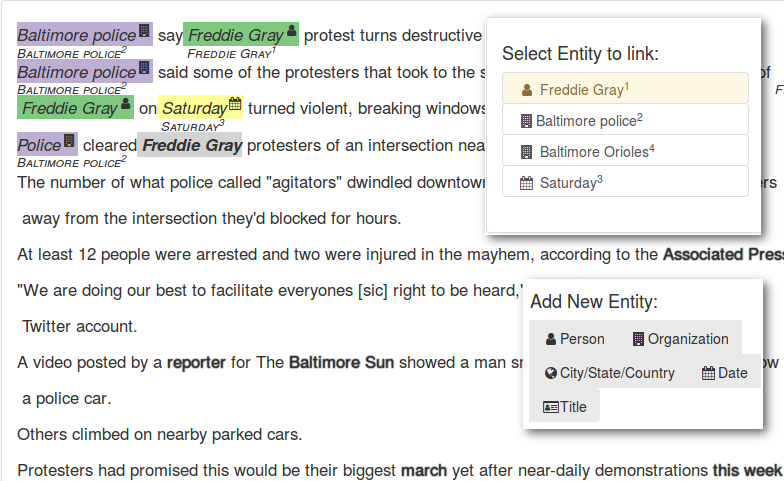
\includegraphics[width=\textwidth]{figures/extraction-interface}
  \caption{\label{fig:entity-interface} Entity detection and linking.}
\end{subfigure}
\caption{\label{fig:interfaces} Screenshots of the annotation interfaces.}
\end{figure*}

\subsection{Evaluating the evaluators}
We begin by analyzing how well crowdworkers perform at verifying relations and exhaustively annotating entities from documents using the annotation interfaces we developed (\figureref{interfaces}).%
%\footnote{%
%  Details of the annotation interfaces used by crowdworkers can be found in \refsec{interface}
%}

\paragraph{Verifying relations}
When verifying relation instances, 
  crowd workers are presented the instance's provenance and are asked to verify
  whether the predicted relation holds between the two mentions and
  whether the mentions are correctly linked if the mention is linked to a Wikipedia entry
  (\figureref{relation-interface}). 
On average, we find that crowdworkers are able to perform this task in about 30 seconds, corresponding to about \$0.10 per instance.
We requested 5 crowdworkers to annotate a small set of 20 relation instances from the 2015 TAC-KBP corpus 
and measured an inter-annotator agreement of \fake{0.90} with 3 crowdworkers and \fake{0.95} with 5.
%\footnote{%
%  Precision is difficult to estimate because the annotations provided TAC-KBP do not specify the subject mention that participates in the relation.
%}
Consequently, we take a majority vote over 3 workers in subsequent experiments.

\paragraph{Annotating entities}
When exhaustively annotating documents for entities and relations,
  crowdworkers begin by identifying every mention span in a document and specifying its type.
  For each mention, they are also asked to identify the canonical mention within the document
  and identify links to Wikipedia pages where possible (\figureref{entity-interface}).
In a separate task, crowdworkers annotate relations between pair of mentions within a sentence.

These interfaces are far more involved: the entity annotation interface takes on average about 13 minutes per document, corresponding to about \$2.60 per document, while the relation annotation interface takes on average about \$2.25 per document.
Because documents vary significantly in length and complexity, we set rewards for each document based on the number of tokens (.75c per token) and mention pairs (5c per pair) respectively.

We compare crowdsourced annotations against those of expert annotators using data from the TAC-KBP 2015 EDL task on 100 documents~\citep{}.
Each document was annotated by at least 7 crowdworkers.
We find that 3 crowdworkers are together identify 92\% of the entity spans identified by expert annotators,
  and 7 crowdworkers together identify 96\%.
When using a token-level majority vote to identify entities, crowdworkers identify about 78\% of the entity spans; this number does not change significantly with additional crowdworkers.
We also measure substantial token-level inter annotator agreement for identifying typed mention spans ($\kappa = 0.83$), canonical mentions ($\kappa = 0.75$) and entity links ($\kappa = 0.75$) with just three workers.
Based on this analysis, we use token-level majority over 3 workers in subsequent experiments.

\subsection{Mock evaluation}
Let us now see how well our new evaluation framework works in practice.

We conduct a mock evaluation using 15,000 newswire documents from 2016 TAC-KBP competition.
We compare the predictions made by three distinct relation extraction systems: a rule-based system, a supervised system and a neural network classifier.
Each system uses Stanford CoreNLP~\citep{} to identify entities and the Illinois Wikifier~\citep{} to perform entity linking. 

\begin{table*}
  \begin{tabular}{l l c c c} \toprule
    Scheme      & System    & $P^e (\pm 95\%)$ & $R^e (\pm 95\%)$ & $\fone{}^e (\pm 95\%)$ \\ \midrule
\multirow{3}{*}{Uncombined} &
  Patterns   & \fake{80.4 $\pm$ 3.0}\% & \fake{10.4 $\pm$ 5.0}\% & \fake{18.41 $\pm$ 4.3}\% \\
& Supervised & \fake{60.4 $\pm$ 3.0}\% & \fake{15.4 $\pm$ 5.0}\% & \fake{24.54 $\pm$ 4.3}\% \\
& Neural     & \fake{20.4 $\pm$ 3.0}\% & \fake{30.4 $\pm$ 5.0}\% & \fake{24.41 $\pm$ 4.3}\% \\ \midrule
\multirow{3}{*}{+ Pooling} &
  Patterns   & \fake{80.4 $\pm$ 3.0}\% & \fake{10.4 $\pm$ 3.0}\% & \fake{18.41 $\pm$ 3.0}\% \\
& Supervised & \fake{60.4 $\pm$ 3.0}\% & \fake{15.4 $\pm$ 3.0}\% & \fake{24.54 $\pm$ 3.0}\% \\
& Neural     & \fake{20.4 $\pm$ 3.0}\% & \fake{30.4 $\pm$ 3.0}\% & \fake{24.41 $\pm$ 3.0}\% \\ \midrule
\multirow{3}{*}{+ Unassessed} &
  Patterns   & \fake{80.4 $\pm$ 2.6}\% & \fake{10.4 $\pm$ 2.7}\% & \fake{18.41 $\pm$ 2.6}\% \\
& Supervised & \fake{60.4 $\pm$ 2.6}\% & \fake{15.4 $\pm$ 2.7}\% & \fake{24.54 $\pm$ 2.6}\% \\
& Neural     & \fake{20.4 $\pm$ 2.6}\% & \fake{30.4 $\pm$ 2.7}\% & \fake{24.41 $\pm$ 2.6}\% \\ \bottomrule
  \end{tabular}
  \caption{\label{tbl:evaluation-results} Results from a mock evaluation.}
\end{table*}

In total, 100 documents were exhaustively annotated for about \$2,000, and 1000 of each systems submissions were annotated at about \$300 each.
\tableref{evaluation-results} presents the results of these systems on the mock evaluation.
%\footnote{A summary of mention-level scores \fake{can be found in the appendix}.}  
% How does cost compare?
% How do absolute scores compare?
Two immediate takeaways are that the precisions of these systems are \fake{on par with their precisions} in the original 2015 evaluation but the 95\% confidence interval is \fake{almost a third as large}.
The recall scores on this evaluation are \fake{a bit smaller than on the 2015 evaluation} and again the 95\% confidence window is \fake{significantly smaller}.
% Score adjustment.
Combining annotation pooling annotations \fake{noticeably reduces} the variance over the uncombined estimation,
while combining the unassessed output \fake{makes a smaller impact}.

% TODO: plot scores per queries as a measure of query variability? How
% do we demonstrate that our artificial query scheme isn't rubbish?
